%%%%%%%%%%%%%%%%%%%%%%%%
%
% $Author: Achal Shakywar $
% $Datum: 15.12.2023  $
% $Pfad: MLProject\ML23-01-Keyword-Spotting-with-an-Arduino-Nano-33-BLE-Sense\report\Images\Domain\DataPreprocessingFlow.tex$
% $Version: 1.0 $
%
% !TeX encoding = utf8
%
%%%%%%%%%%%%%%%%%%%%%%%%

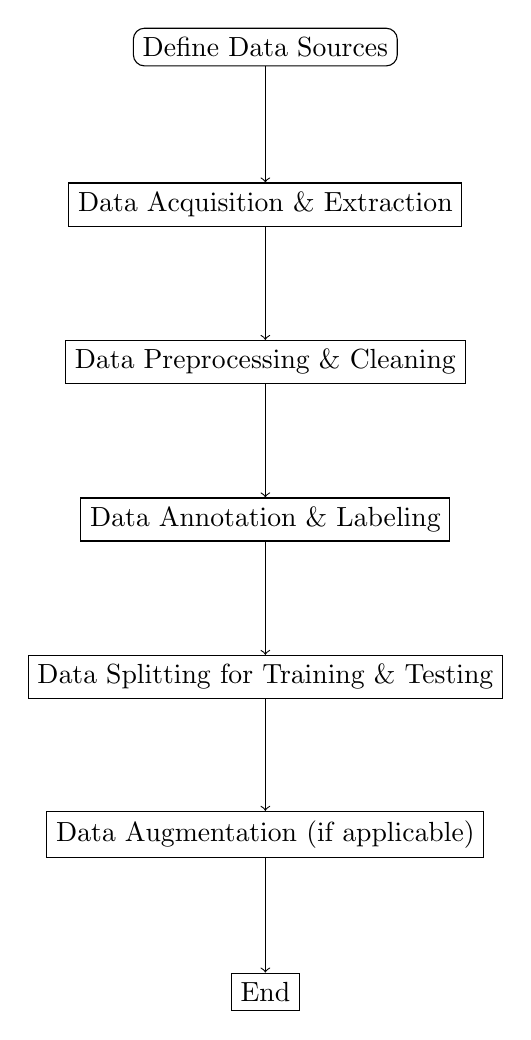
\begin{tikzpicture}[node distance=2cm, auto]
    % Nodes
    \node (sources) [draw, rounded corners] {Define Data Sources};
    \node (acquisition) [draw, below of=sources] {Data Acquisition \& Extraction};
    \node (preprocessing) [draw, below of=acquisition] {Data Preprocessing \& Cleaning};
    \node (annotation) [draw, below of=preprocessing] {Data Annotation \& Labeling};
    \node (splitting) [draw, below of=annotation] {Data Splitting for Training \& Testing};
    \node (augmentation) [draw, below of=splitting] {Data Augmentation (if applicable)};
    \node (end) [draw, below of=augmentation] {End};

    % Arrows
    \draw [->] (sources) -- (acquisition);
    \draw [->] (acquisition) -- (preprocessing);
    \draw [->] (preprocessing) -- (annotation);
    \draw [->] (annotation) -- (splitting);
    \draw [->] (splitting) -- (augmentation);
    \draw [->] (augmentation) -- (end);

\end{tikzpicture}

